% Options for packages loaded elsewhere
\PassOptionsToPackage{unicode}{hyperref}
\PassOptionsToPackage{hyphens}{url}
\PassOptionsToPackage{dvipsnames,svgnames,x11names}{xcolor}
%
\documentclass[
  letterpaper,
  DIV=11,
  numbers=noendperiod]{scrartcl}

\usepackage{amsmath,amssymb}
\usepackage{iftex}
\ifPDFTeX
  \usepackage[T1]{fontenc}
  \usepackage[utf8]{inputenc}
  \usepackage{textcomp} % provide euro and other symbols
\else % if luatex or xetex
  \usepackage{unicode-math}
  \defaultfontfeatures{Scale=MatchLowercase}
  \defaultfontfeatures[\rmfamily]{Ligatures=TeX,Scale=1}
\fi
\usepackage{lmodern}
\ifPDFTeX\else  
    % xetex/luatex font selection
\fi
% Use upquote if available, for straight quotes in verbatim environments
\IfFileExists{upquote.sty}{\usepackage{upquote}}{}
\IfFileExists{microtype.sty}{% use microtype if available
  \usepackage[]{microtype}
  \UseMicrotypeSet[protrusion]{basicmath} % disable protrusion for tt fonts
}{}
\makeatletter
\@ifundefined{KOMAClassName}{% if non-KOMA class
  \IfFileExists{parskip.sty}{%
    \usepackage{parskip}
  }{% else
    \setlength{\parindent}{0pt}
    \setlength{\parskip}{6pt plus 2pt minus 1pt}}
}{% if KOMA class
  \KOMAoptions{parskip=half}}
\makeatother
\usepackage{xcolor}
\setlength{\emergencystretch}{3em} % prevent overfull lines
\setcounter{secnumdepth}{-\maxdimen} % remove section numbering
% Make \paragraph and \subparagraph free-standing
\ifx\paragraph\undefined\else
  \let\oldparagraph\paragraph
  \renewcommand{\paragraph}[1]{\oldparagraph{#1}\mbox{}}
\fi
\ifx\subparagraph\undefined\else
  \let\oldsubparagraph\subparagraph
  \renewcommand{\subparagraph}[1]{\oldsubparagraph{#1}\mbox{}}
\fi

\usepackage{color}
\usepackage{fancyvrb}
\newcommand{\VerbBar}{|}
\newcommand{\VERB}{\Verb[commandchars=\\\{\}]}
\DefineVerbatimEnvironment{Highlighting}{Verbatim}{commandchars=\\\{\}}
% Add ',fontsize=\small' for more characters per line
\usepackage{framed}
\definecolor{shadecolor}{RGB}{100,100,100}
\newenvironment{Shaded}{\begin{snugshade}}{\end{snugshade}}
\newcommand{\KeywordTok}[1]{\textcolor[rgb]{0.00,0.13,1.00}{#1}}
\newcommand{\ClassTok}[1]{\textcolor[rgb]{0.27,0.56,0.65}{#1}}
\newcommand{\OperatorTok}[1]{\textcolor[rgb]{0.00,0.00,0.00}{#1}}
\newcommand{\VariableTok}[1]{\textcolor[rgb]{0.00,0.06,0.50}{#1}}
\newcommand{\ValueTok}[1]{\textcolor[rgb]{0.13,0.57,0.41}{#1}}
\newcommand{\FunctionTok}[1]{\textcolor[rgb]{0.47,0.37,0.15}{#1}}
\newcommand{\IDETok}[1]{\textcolor[rgb]{0.58,0.58,0.58}{#1}}
\newcommand{\NormalTok}[1]{\textcolor[rgb]{0.00,0.06,0.50}{#1}}
\newcommand{\CommentTok}[1]{\textcolor[rgb]{0.00,0.50,0.00}{#1}}
\newcommand{\StringTok}[1]{\textcolor[rgb]{0.70,0.27,0.27}{#1}}


\providecommand{\tightlist}{%
  \setlength{\itemsep}{0pt}\setlength{\parskip}{0pt}}\usepackage{longtable,booktabs,array}
\usepackage{calc} % for calculating minipage widths
% Correct order of tables after \paragraph or \subparagraph
\usepackage{etoolbox}
\makeatletter
\patchcmd\longtable{\par}{\if@noskipsec\mbox{}\fi\par}{}{}
\makeatother
% Allow footnotes in longtable head/foot
\IfFileExists{footnotehyper.sty}{\usepackage{footnotehyper}}{\usepackage{footnote}}
\makesavenoteenv{longtable}
\usepackage{graphicx}
\makeatletter
\def\maxwidth{\ifdim\Gin@nat@width>\linewidth\linewidth\else\Gin@nat@width\fi}
\def\maxheight{\ifdim\Gin@nat@height>\textheight\textheight\else\Gin@nat@height\fi}
\makeatother
% Scale images if necessary, so that they will not overflow the page
% margins by default, and it is still possible to overwrite the defaults
% using explicit options in \includegraphics[width, height, ...]{}
\setkeys{Gin}{width=\maxwidth,height=\maxheight,keepaspectratio}
% Set default figure placement to htbp
\makeatletter
\def\fps@figure{htbp}
\makeatother
\newlength{\cslhangindent}
\setlength{\cslhangindent}{1.5em}
\newlength{\csllabelwidth}
\setlength{\csllabelwidth}{3em}
\newlength{\cslentryspacingunit} % times entry-spacing
\setlength{\cslentryspacingunit}{\parskip}
\newenvironment{CSLReferences}[2] % #1 hanging-ident, #2 entry spacing
 {% don't indent paragraphs
  \setlength{\parindent}{0pt}
  % turn on hanging indent if param 1 is 1
  \ifodd #1
  \let\oldpar\par
  \def\par{\hangindent=\cslhangindent\oldpar}
  \fi
  % set entry spacing
  \setlength{\parskip}{#2\cslentryspacingunit}
 }%
 {}
\usepackage{calc}
\newcommand{\CSLBlock}[1]{#1\hfill\break}
\newcommand{\CSLLeftMargin}[1]{\parbox[t]{\csllabelwidth}{#1}}
\newcommand{\CSLRightInline}[1]{\parbox[t]{\linewidth - \csllabelwidth}{#1}\break}
\newcommand{\CSLIndent}[1]{\hspace{\cslhangindent}#1}

\KOMAoption{captions}{tableheading}
\makeatletter
\makeatother
\makeatletter
\makeatother
\makeatletter
\@ifpackageloaded{caption}{}{\usepackage{caption}}
\AtBeginDocument{%
\ifdefined\contentsname
  \renewcommand*\contentsname{Table of contents}
\else
  \newcommand\contentsname{Table of contents}
\fi
\ifdefined\listfigurename
  \renewcommand*\listfigurename{List of Figures}
\else
  \newcommand\listfigurename{List of Figures}
\fi
\ifdefined\listtablename
  \renewcommand*\listtablename{List of Tables}
\else
  \newcommand\listtablename{List of Tables}
\fi
\ifdefined\figurename
  \renewcommand*\figurename{Figure}
\else
  \newcommand\figurename{Figure}
\fi
\ifdefined\tablename
  \renewcommand*\tablename{Table}
\else
  \newcommand\tablename{Table}
\fi
}
\@ifpackageloaded{float}{}{\usepackage{float}}
\floatstyle{ruled}
\@ifundefined{c@chapter}{\newfloat{codelisting}{h}{lop}}{\newfloat{codelisting}{h}{lop}[chapter]}
\floatname{codelisting}{Listing}
\newcommand*\listoflistings{\listof{codelisting}{List of Listings}}
\makeatother
\makeatletter
\@ifpackageloaded{caption}{}{\usepackage{caption}}
\@ifpackageloaded{subcaption}{}{\usepackage{subcaption}}
\makeatother
\makeatletter
\@ifpackageloaded{tcolorbox}{}{\usepackage[skins,breakable]{tcolorbox}}
\makeatother
\makeatletter
\makeatother
\makeatletter
\makeatother
\ifLuaTeX
  \usepackage{selnolig}  % disable illegal ligatures
\fi
\IfFileExists{bookmark.sty}{\usepackage{bookmark}}{\usepackage{hyperref}}
\IfFileExists{xurl.sty}{\usepackage{xurl}}{} % add URL line breaks if available
\urlstyle{same} % disable monospaced font for URLs
\hypersetup{
  pdftitle={Poincaré and SimBio: a versatile and extensible Python ecosystem for modeling systems.},
  colorlinks=true,
  linkcolor={blue},
  filecolor={Maroon},
  citecolor={Blue},
  urlcolor={Blue},
  pdfcreator={LaTeX via pandoc}}

\usepackage{authblk}
\renewcommand\Affilfont{\small}

\title{Poincaré and SimBio: a versatile and extensible Python ecosystem
for modeling systems.}
\author[1,2]{Mauro Silberberg}
\author[3]{Henning Hermjakob}
\author[3]{Rahuman S. Malik-Sheriff}
\author[1,2]{Hernán E. Grecco}
\affil[1]{Universidad de Buenos Aires, Facultad de Ciencias Exactas y Naturales, Departamento de Física. Buenos Aires, Argentina.}
\affil[2]{CONICET - Universidad de Buenos Aires, Instituto de Física de Buenos Aires (IFIBA). Buenos Aires, Argentina}
\affil[3]{European Bioinformatics Institute, European Molecular Biology Laboratory (EMBL-EBI), Wellcome Trust Genome Campus, Cambridge, UK}
\date{}

\begin{document}
\maketitle
\begin{abstract}
Chemical Reaction Networks (CRNs) play a pivotal role in diverse fields
such as systems biology, biochemistry, chemical engineering, and
epidemiology. High-level modelling of CRNs enables various simulation
approaches, including deterministic and stochastic methods. However,
existing Python tools for CRN modelling typically wrap external C/C++
libraries for modelling and simulation, limiting their extensibility and
integration with the broader Python ecosystem. In response, we developed
Poincaré and SimBio, two novel Python packages for the definition and
simulation of dynamical systems and CRNs. Poincaré serves as a
foundation for dynamical system modelling, while SimBio extends this
functionality to CRNs, including support for the Systems Biology Markup
Language (SBML). Poincaré and SimBio are developed as pure Python
packages enabling users to easily extend their simulation capabilities
by writing new or leveraging other Python packages. Moreover, this does
not compromise the performance, as code can be Just-In-Time compiled
with Numba. Our benchmark tests using curated models from the BioModels
repository, demonstrate that these tools may provide a potentially
superior performance advantage, compared to other existing tools.
Additionally, to ensure a user-friendly experience, our packages use
standard typed modern Python syntax that provides a seamless integration
with Integrated Development Environments (IDEs). Python-centric approach
significantly enhances code analysis, error detection, and refactoring
capabilities, positioning Poincaré and SimBio as valuable tools for the
modelling community.
\end{abstract}
\ifdefined\Shaded\renewenvironment{Shaded}{\begin{tcolorbox}[sharp corners, frame hidden, borderline west={3pt}{0pt}{shadecolor}, breakable, boxrule=0pt, enhanced]}{\end{tcolorbox}}\fi

\hypertarget{introduction}{%
\section{Introduction}\label{introduction}}

Chemical Reaction Networks (CRNs) are a fundamental concept of modelling
in numerous fields including systems biology, biochemistry, chemical
engineering and epidemiology. They are comprised of a set of chemical
species or biological entities and representation of complex interaction
and transformation between them through a series reactions. These
systems can be modelled and simulated through multiple approaches:
deterministic Ordinary Differential Equations (ODEs) to model
macroscopic behavior, Stochastic Differential Equations (SDEs) to model
microscopic fluctuations, and jump processes (Gillespie-like
simulations) to account for the discreteness of populations. Instead of
directly writing the equations for each of these formulations which is
error-prone and difficult to reuse, these models can be written in a
higher-level description that can be compiled for these different types
of simulations.

Several tools already exist for defining and simulating CRNs.
BioSimulators.org (Shaikh et al. 2022), a registry of simulation tools,
list at least 15 Python software including COPASI (Hoops et al. 2006),
Tellurium (Choi et al. 2018) and PySB (Lopez et al. 2013). COPASI is a
standalone software with a GUI for defining and simulating models. It's
widely used for its user-friendly interface and comprehensive features.
There are also python bindings and interfaces for COPASI to allow
advanced scripting. Tellurium is a Python-based modeling environment,
however, it uses a C++ library called libRoadRunner in the backend to
simulate models. PySB is a Python library that created a DSL using
standard Python to define models which are then compiled to ODE using a
Perl library called BioNetGen (L. A. Harris et al. 2016).

One limitation of these tools is that they are not extensible from
Python, as they are not fully Python packages but wrap libraries in
other languages to do the simulation. While they enable model definition
and simulation control via Python scripts, they don't fully leverage
Python's extensive package ecosystem. For example, in COPASI, users are
restricted to predefined distributions for Random Parameter Scans and
cannot utilize the diverse distributions available in
\texttt{scipy.stats}. Similarly, Tellurium doesn't allow the use of
Python solvers, as adding new integrators requires C++ implementation.

\begin{figure}[t]

\begin{minipage}[t]{\linewidth}

{\centering 

\begin{CodeInput}
\begin{Highlighting}[]
\KeywordTok{from} \ClassTok{poincare} \KeywordTok{import} \ClassTok{Derivative}, \ClassTok{System}, \ClassTok{Variable}, \FunctionTok{initial}
\end{Highlighting}
\end{CodeInput}

}

\end{minipage}%
\newline
\begin{minipage}[t]{\linewidth}

{\centering

\begin{minipage}[c]{0.6\linewidth}

{\centering 

\begin{CodeInput}
\begin{Highlighting}[]
\KeywordTok{class} \ClassTok{Decay}\KeywordTok{(}\ClassTok{System}\KeywordTok{)}\OperatorTok{:}
    \VariableTok{x}\OperatorTok{:} \ClassTok{Variable} \OperatorTok{=} \FunctionTok{initial}\KeywordTok{(\VariableTok{default}\OperatorTok{=}\ValueTok{1})}
    \VariableTok{eq} \OperatorTok{=} \VariableTok{x}.\FunctionTok{derive}\KeywordTok{()} \OperatorTok{\textless{}\textless{}} \OperatorTok{-}\VariableTok{x}
\end{Highlighting}
\end{CodeInput}

}

\end{minipage}%
%
\begin{minipage}[c]{0.2\linewidth}

{\centering 

\[
\frac{dx}{dt} = -x
\]

}

\end{minipage}%
%
\begin{minipage}[c]{0.2\linewidth}

{\centering 

\[
x(0) = 1
\]

}

\end{minipage}%

\subcaption{\label{fig-first-order}First-order system of an exponential decay. The variable
\texttt{x} stores the initial condition for \(x\), and the variable
\texttt{eq} stores the rate equation for \(x\).}

}

\end{minipage}%
\newline
\begin{minipage}[t]{\linewidth}

{\centering 

\begin{minipage}[c]{0.6\linewidth}

{\centering 

\begin{CodeInput}
\begin{Highlighting}[]
\KeywordTok{class} \ClassTok{Oscillator}\KeywordTok{(}\ClassTok{System}\KeywordTok{)}\OperatorTok{:}
    \VariableTok{x}: \ClassTok{Variable} \OperatorTok{=} \FunctionTok{initial}\KeywordTok{(\VariableTok{default}\OperatorTok{=}\ValueTok{1})}
    \VariableTok{v}: \ClassTok{Derivative} \OperatorTok{=} \VariableTok{x}.\FunctionTok{derive}\KeywordTok{(\VariableTok{initial}\OperatorTok{=}\ValueTok{0})}
    \VariableTok{eq} \OperatorTok{=} \VariableTok{v}.\FunctionTok{derive}\KeywordTok{()} \OperatorTok{\textless{}\textless{}} \OperatorTok{-}\VariableTok{x}
\end{Highlighting}
\end{CodeInput}

}

\end{minipage}%
%
\begin{minipage}[c]{0.2\linewidth}

{\centering 

\[
\frac{d^2x}{dt^2} = -x
\]

}

\end{minipage}%
%
\begin{minipage}[c]{0.2\linewidth}

{\centering 

\[
\begin{cases}
    x(0) &= 1 \\
    \frac{dx}{dt}(0) &= 0
\end{cases}
\]

}

\end{minipage}%

\subcaption{\label{fig-second-order}Second-order system of an harmonic oscillator, where the
variable \texttt{v} stores the derivative \(\frac{dx}{dt}\) and the rate
equation is specified for the derivative \texttt{v}.}

}

\end{minipage}%
\newline
\begin{minipage}[t]{\linewidth}

{\centering 

\begin{minipage}[c]{0.6\linewidth}

{\centering 

\begin{CodeInput}
\begin{Highlighting}[]
\KeywordTok{class} \ClassTok{BigModel}\KeywordTok{(}\ClassTok{System}\KeywordTok{)}:
    \VariableTok{x}: \ClassTok{Variable} \OperatorTok{=} \FunctionTok{initial}\KeywordTok{(\VariableTok{default}\OperatorTok{=}\ValueTok{1})}
    \VariableTok{linked} \OperatorTok{=} \ClassTok{Decay}\KeywordTok{(\VariableTok{x}\OperatorTok{=}\VariableTok{x})}
    \VariableTok{independent} \OperatorTok{=} \ClassTok{Decay}\KeywordTok{(\VariableTok{x}\OperatorTok{=}\ValueTok{2})}
\end{Highlighting}
\end{CodeInput}

}

\end{minipage}%
%
\begin{minipage}[c]{0.2\linewidth}

{\centering 

\[
\begin{cases}
    \frac{dx}{dt} = -x \\
    \frac{dx_{ind}}{dt} = -x_{ind}
\end{cases}
\]

}

\end{minipage}%
%
\begin{minipage}[c]{0.2\linewidth}

{\centering 

\[
\begin{cases}
    x(0) &= 1 \\
    x_{ind}(0) &= 2
\end{cases}
\]

}

\end{minipage}%

\subcaption{\label{fig-composition}First-order system of two exponential decays by composition of
the \texttt{Decay} system. The subsystem \texttt{linked} has a reference
to the outer variable \texttt{x}, while the subsystem
\texttt{independent} defines a new variable with initial condition $2$,
which on the corresponding mathematical expression was named \(x_{ind}\).}

}

\end{minipage}%

\caption{\label{fig-poincare}Code and corresponding mathematical
expressions for different systems.}

\end{figure}


Another challenge is the way models are written. Many tools use a Domain
Specific Language (DSL) for coding, and support the System Biology
Markup Language (SBML) as an exchange format (Hucka et al., n.d.), as
direct SBML coding is impractical. A DSL allows reuse of code in
different programming environments, but it will not be recognized by
default in Integrated Development Environments (IDEs). Therefore DSLs
cannot provide the development experience such as syntax highlighting,
code completion, refactoring, and static analysis, unless such support
is specifically developed. Tellurium uses a Domain Specific Language
(DSL) called Antimony (Smith et al. 2009), which can be translated to
SBML. An extension for Visual Studio Code was developed, but its
maintenance could be demanding task for the systems biology community.
PySB, using Python's dynamic nature, created a DSL within Python. By
default, it uses global state to create species and parameters, without
assigning them to Python variables or adding them explicitly to the
model, but this approach is not fully compatible with IDEs, affecting
the development experience.

To overcome these limitations, we developed poincaré and SimBio,
open-source Python packages for defining and simulating systems.
Poincaré allows defining differential equation systems, while SimBio
builds on it for defining reaction networks. They are focused on
providing an ergonomic experience to end-users by integrating well with
IDEs and static analysis tools through the use of standard modern Python
syntax. Since they are coded in Python, every part from model definition
to simulation can be extended from Python syntax. Being the first-ever
pure Python packages for systems modelling, they offer extensive
extensibility, from simple tasks like reusing integrators defined in
other packages, to complex ones like altering the compilation process to
leverage some structure in the equations. For example, using a for-loop
in the compiled equations could improve the runtime performance if there
is some repetitive structure in the system, as happens in spatial
modelling. The models built using these packages can be introspected to
create other representations, such as graphs connecting species and/or
reactions, or tables with parameters or equations. Furthermore, they
have a modular architecture with a clear separation of concerns, making
it easier to maintain or to contribute new code, which is beneficial for
developers and maintainers. We showcased the reliability of these tools
by benchmarking them against the simulation results from other tools. We
also highlighted the substantial performance improvements our tools
offer, as this is crucial for construction and simulation of models of
whole cells and organisms, which necessitate the simulation of
significantly large-scale models.

\hypertarget{results}{%
\section{Results}\label{results}}

\begin{figure}[t]

\begin{minipage}[b]{0.50\linewidth}
{
    \centering 
    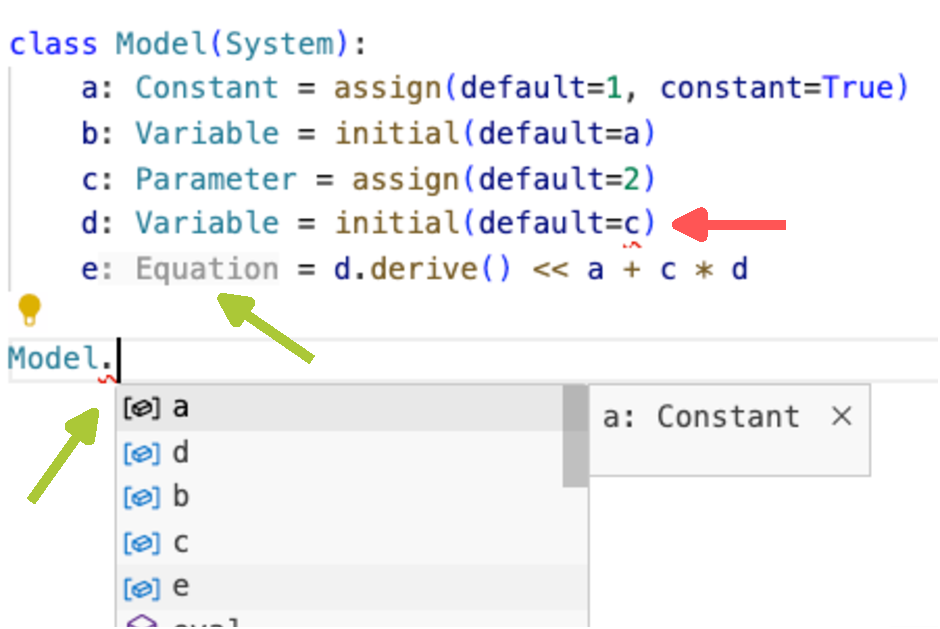
\includegraphics{src/ide/ide1.pdf}
}
\end{minipage}%
%
\begin{minipage}[b]{0.50\linewidth}
{
    \centering
    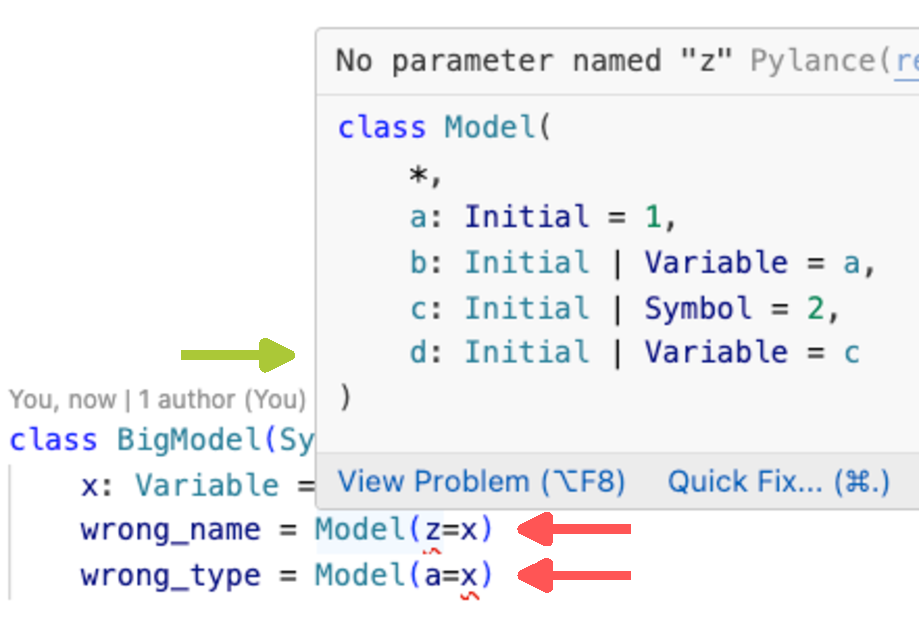
\includegraphics{src/ide/ide2.pdf}
}
\end{minipage}%

\caption{
    \label{fig-ide}
    Screenshots of Visual Studio Code showing
    tooltips (green arrows) and
    highlighted type errors (red arrows).
    On the left,
    we show that \texttt{a},
    a \texttt{Constant} assigned with \texttt{assign(...,\ constant=True)},
    can be used for \texttt{Variable b}'s initial condition.
    Instead,
    it is flagged as a type error (red underlining)
    when using \texttt{c}, a \texttt{Parameter},
    for \texttt{Variable d}'s initial condition,
    The IDE automatically recognizes \texttt{e} as an \texttt{Equation},
    and provides autocompletion of the \texttt{Model}'s components.
    A tooltip is shown when composing models (green arrow, right),
    which show the expected variables and their default values.
    The IDE highlights wrong names (\texttt{z} is not a name in \texttt{Model})
    and mismatched types (\texttt{x} is \texttt{Variable} and \texttt{a} must be a number or a \texttt{Constant})
}

\end{figure}


Modular code architecture makes code reusable, extensible, and easier to
maintain. Therefore, we split the code to define and simulate reaction
systems into three Python packages: symbolite, to create symbolic
expressions; poincaré, to define dynamical systems; and simbio, to
define reaction systems and interface with systems biology standards
such as SBML. These are pure Python packages with standard dependencies
from the PyData scientific stack such as NumPy (C. R. Harris et al.
2020) and pandas (McKinney 2010). They are published in PyPI (the Python
Package Index), where links to the source code and documentation hosted
in GitHub can be found, and can be easily installed with
\texttt{pip\ install\ \textless{}package\_name\textgreater{}}.

Symbolite is a lightweight symbolics package to create algebraic
mathematical expressions. Symbolite expressions can be inspected and
compiled to various backends. Currently, we have implementations for
NumPy (C. R. Harris et al. 2020); Numba (Lam, Pitrou, and Seibert 2015),
a Just-in-Time (JIT) compiler to LLVM; SymPy (Meurer et al. 2017), a
library for symbolic mathematics; and JAX (Bradbury et al. 2018), a
library that support automatic differentiation and compilation to GPUs
and TPUs. Symbolite is designed to facilitate the easy integration of
new backends.

\hypertarget{versatile-modelling-and-simulation-of-dynamical-systems-with-poincaruxe9}{%
\subsection{Versatile modelling and simulation of dynamical systems with
Poincaré}\label{versatile-modelling-and-simulation-of-dynamical-systems-with-poincaruxe9}}

\begin{figure}[t]

\begin{minipage}[t]{\linewidth}

{\centering 

\begin{Shaded}
\begin{Highlighting}[]
\ImportTok{import}\NormalTok{ numpy }\ImportTok{as}\NormalTok{ np}
\ImportTok{from}\NormalTok{ poincare }\ImportTok{import}\NormalTok{ Simulator}

\NormalTok{sim }\OperatorTok{=}\NormalTok{ Simulator(Oscillator)}
\NormalTok{df }\OperatorTok{=}\NormalTok{ sim.solve(save\_at}\OperatorTok{=}\NormalTok{np.linspace(}\DecValTok{0}\NormalTok{, }\DecValTok{5}\NormalTok{, }\DecValTok{101}\NormalTok{))}
\end{Highlighting}
\end{Shaded}

}

\end{minipage}%
\newline
\begin{minipage}[t]{0.45\linewidth}

{\centering 

\begin{Shaded}
\begin{Highlighting}[]
\NormalTok{df.head()}
\end{Highlighting}
\end{Shaded}

\begin{longtable}[]{@{}lll@{}}
\toprule\noalign{}
& x & v \\
time & & \\
\midrule\noalign{}
\endhead
\bottomrule\noalign{}
\endlastfoot
0.00 & 1.000000 & 0.000000 \\
0.05 & 0.998750 & -0.049979 \\
0.10 & 0.995005 & -0.099835 \\
0.15 & 0.988772 & -0.149440 \\
0.20 & 0.980069 & -0.198672 \\
\end{longtable}

}

\end{minipage}%
\hfill
\begin{minipage}[t]{0.45\linewidth}

{\centering 

\begin{Shaded}
\begin{Highlighting}[]
\NormalTok{df.plot()}\OperatorTok{;}
\end{Highlighting}
\end{Shaded}

\begin{figure}[H]

{\centering 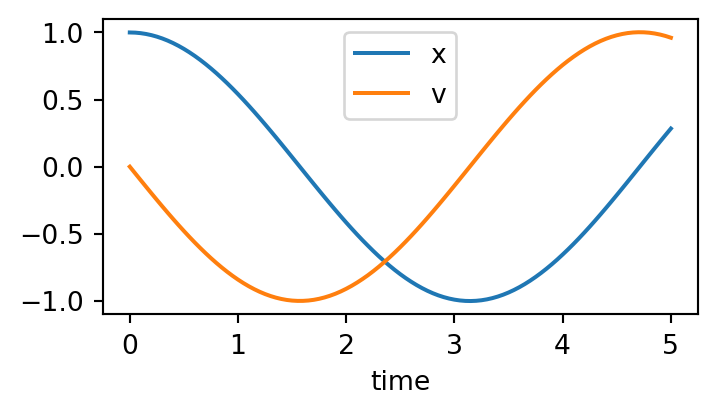
\includegraphics{article_files/figure-latex/cell-9-output-1.pdf}

}

\end{figure}

}

\end{minipage}%

\caption{\label{fig-sim}Simulation of the \texttt{Oscillator} system
from Figure~\ref{fig-second-order}. The output is a
\texttt{pandas.DataFrame} with a column for each variable and the time
as index. It is inspected and plotted with the \texttt{pandas} methods.}

\end{figure}


Poincare is a package to define and simulate dynamical systems. It
provides a \texttt{System} class, where one can define
\texttt{Constant}s, \texttt{Parameter}s, \texttt{Variable}s, and create
equations linking a variable's derivative with an expression
(Figure~\ref{fig-first-order}). It also allows to define higher-order
systems by assigning an initial condition to a \texttt{Derivative}
(Figure~\ref{fig-second-order}).

Utilizing classes for system definition offers several advantages:

\begin{enumerate}
\def\labelenumi{\arabic{enumi}.}
\tightlist
\item
  The variable name to which a component is assigned can be
  automatically saved in the component for introspection (i.e.,
  \texttt{Oscilator.x.name\ ==\ "x"}),
\item
  It provides a namespace such that allows to easily define of multiple
  independent models in the same script,
\item
  It allows IDEs to provide autocomplete and refactoring capabilities
  (\texttt{Oscillator.\textless{}TAB\textgreater{}} shows \texttt{x},
  \texttt{v} and \texttt{eq}),
\item
  It allows creation of instances which can be composed into a bigger
  model (Figure~\ref{fig-composition}).
\end{enumerate}

\begin{figure}[t]

\begin{minipage}[t]{\linewidth}

{\centering 

\begin{CodeInput}
\begin{Highlighting}[]
\KeywordTok{from}\ClassTok{ simbio }\KeywordTok{import}\ClassTok{ Compartment, MassAction, Species, RateLaw, \FunctionTok{initial}}
\end{Highlighting}
\end{CodeInput}

}

\end{minipage}%
\newline
\begin{minipage}[t]{\linewidth}

{\centering 

\begin{minipage}[c]{0.60\linewidth}

{\centering 

\begin{CodeInput}
\begin{Highlighting}[]
\KeywordTok{class}\ClassTok{ Model}\KeywordTok{(}\ClassTok{Compartment}\KeywordTok{)}:
    \CommentTok{"""2A {-}\textgreater{} B"""}

\VariableTok{    A}: \ClassTok{Species }\OperatorTok{=}\FunctionTok{ initial}\KeywordTok{(}\VariableTok{default}\OperatorTok{=}\ValueTok{1}\KeywordTok{)}
\VariableTok{    B}: \ClassTok{Species }\OperatorTok{=}\FunctionTok{ initial}\KeywordTok{(}\VariableTok{default}\OperatorTok{=}\ValueTok{0}\KeywordTok{)}
\VariableTok{    r }\OperatorTok{=}\ClassTok{ RateLaw}\KeywordTok{(}
\VariableTok{        reactants}\OperatorTok{=}\KeywordTok{[}\ValueTok{2} \OperatorTok{*}\VariableTok{ A}\KeywordTok{]},
\VariableTok{        products}\OperatorTok{=}\NormalTok{\KeywordTok{[}B\KeywordTok{]},}
\VariableTok{        rate}\OperatorTok{=}\ValueTok{1}\NormalTok{,}
\KeywordTok{    )}
\end{Highlighting}
\end{CodeInput}

}

\end{minipage}%
%
\begin{minipage}[c]{0.40\linewidth}

{\centering 

\[
\begin{cases}
    \frac{dA}{dt} = -2 \\
    \frac{dB}{dt} = +1
\end{cases}
\begin{cases}
    A(0) &= 1 \\
    B(0) &= 0
\end{cases}
\]

}

\end{minipage}%

}

\end{minipage}%
\newline
\begin{minipage}[t]{\linewidth}

{\centering 

\begin{minipage}[c]{0.60\linewidth}

{\centering 

\begin{CodeInput}
\begin{Highlighting}[]
\KeywordTok{class}\ClassTok{ Model}\KeywordTok{(}\ClassTok{Compartment}\KeywordTok{)}:
    \CommentTok{"""2A {-}\textgreater{} B"""}

\VariableTok{    A}: \ClassTok{Species }\OperatorTok{=}\FunctionTok{ initial}\KeywordTok{(}\VariableTok{default}\OperatorTok{=}\ValueTok{1}\KeywordTok{)}
\VariableTok{    B}: \ClassTok{Species }\OperatorTok{=}\FunctionTok{ initial}\KeywordTok{(}\VariableTok{default}\OperatorTok{=}\ValueTok{0}\KeywordTok{)}
\VariableTok{    r }\OperatorTok{=}\ClassTok{ MassAction}\KeywordTok{(}
\VariableTok{        reactants}\OperatorTok{=}\KeywordTok{[}\ValueTok{2} \OperatorTok{*}\VariableTok{ A}\KeywordTok{]},
\VariableTok{        products}\OperatorTok{=}\NormalTok{\KeywordTok{[}B\KeywordTok{]},}
\VariableTok{        rate}\OperatorTok{=}\ValueTok{1}\NormalTok{,}
\KeywordTok{    )}
\end{Highlighting}
\end{CodeInput}

}

\end{minipage}%
%
\begin{minipage}[c]{0.40\linewidth}

{\centering 

\[
\begin{cases}
    \frac{dA}{dt} = -2 A^2 \\
    \frac{dB}{dt} = +1 A^2
\end{cases}
\begin{cases}
    A(0) &= 1 \\
    B(0) &= 0
\end{cases}
\]

}

\end{minipage}%

}

\end{minipage}%

\caption{\label{fig-simbio}A reaction system for species \(A\) and \(B\)
with initial conditions \(1\) and \(0\), respectively. A single reaction
transforming \(2A\) into \(B\) is saved in variable \texttt{r}. The rate
\(1\) is specified directly for \texttt{RateLaw}, and is proportional to
the reactants for \texttt{MassAction}.}

\end{figure}


For this last point, IDEs that support \texttt{dataclass\_transform} (De
Bonte and Traut 2021) can provide a tooltip with the expected signature
(Figure~\ref{fig-composition}). This requires the use of type
annotations which play a more significant role in static type checking,
as they can help to identify errors before running the code. For
instance, to parameterize the initial conditions of variables we have to
use a \texttt{Constant}. If we try to use a \texttt{Parameter}, which
could be a time-dependent expression, it is flagged as a type error
(Figure~\ref{fig-ide}).

To simulate a system, we created a \texttt{Simulator} instance
(Figure~\ref{fig-sim}), which compiles a given system and interfaces
with solvers. By default, it creates a first-order ordinary differential
equation (ODE) system using \texttt{numpy} as a backend. This can be
easily switched to other solvers. The Simulator wraps the output in a
\texttt{pandas.DataFrame}, which can be easily plotted with the standard
\texttt{plot} method.

Switching backends to \texttt{"numba"} can improve model runtime on a
factor up to x30 or more for big or long running models, however incurs
in a compile time penalty for the first run which must be taken into
account.

\hypertarget{extensible-definition-of-reaction-networks-using-simbio}{%
\subsection{Extensible definition of reaction networks using
SimBio}\label{extensible-definition-of-reaction-networks-using-simbio}}

For the reaction networks, our focus is on first-order differential
equations that describe the rate of change of species. SimBio simplifies
the definition of these network models by introducing \texttt{Species},
which consists of a \texttt{poincare.Variable} and a stoichiometric
number, and \texttt{RateLaw}, a construct that converts reactants into
products taking into account the stoichiometry
(Figure~\ref{fig-simbio}). Additionally, SimBio features
\texttt{MassAction}, a subclass of \texttt{RateLaw}, which intuitively
incorporates reactants into the rate law (Figure~\ref{fig-simbio}).

Several commonly used reactions are predefined as \texttt{MassAction}
subclasses, such as \texttt{MichaelisMenten}
(\(S + E \leftrightarrow ES \rightarrow P + E\)) and its approximate
form without the intermediate species \(ES\), and it is also simple to
implement your own as subclasses of \texttt{RateLaw} or
\texttt{MassAction}. Additionally, SimBio supports importing from and
exporting to SBML, and downloading them directly from BioModels
(Malik-Sheriff et al. 2020) (Figure~\ref{fig-simbio-io}).

\begin{figure}[t]

\begin{minipage}[t]{\linewidth}

{\centering 

\begin{Shaded}
\begin{Highlighting}[]
\KeywordTok{from}\ClassTok{ simbio.io }\KeywordTok{import}\ClassTok{ biomodels, sbml}

\VariableTok{model }\OperatorTok{=}\ClassTok{ sbml}.\FunctionTok{load}\KeywordTok{(}\StringTok{"repressilator.sbml"}\KeywordTok{)}  \CommentTok{\# from existing SBML file}
\VariableTok{model }\OperatorTok{=}\ClassTok{ biomodels}.\FunctionTok{load\_model}\KeywordTok{(}\StringTok{"BIOMD12"}\KeywordTok{)}  \CommentTok{\# from BioModels}
\VariableTok{model}
\end{Highlighting}
\end{Shaded}

\begin{longtable}{@{}lll@{}}
    \multicolumn{3}{l}{Elowitz2000 - Repressilator} \\
    \toprule\noalign{}
    type & total & names \\
    \midrule\noalign{}
    \endhead
    \bottomrule\noalign{}
    \endlastfoot
    variables  &  6 & PX, PY, PZ, X, Y, Z \\
    parameters & 17 & cell, beta, alpha0, alpha, eff, n, KM, tau\_mRNA, tau\_prot, ... \\
    equations  & 12 & Reaction1, Reaction2, Reaction3, Reaction4, Reaction5, ... \\
\end{longtable}

}

\end{minipage}%

\caption{\label{fig-simbio-io}Creation of a model from a local SBML file
or one uploaded to BioModels.}

\end{figure}


\hypertarget{reproducibility-and-performance}{%
\subsection{Reproducibility and
performance}\label{reproducibility-and-performance}}

\begin{figure}[t]

{\centering 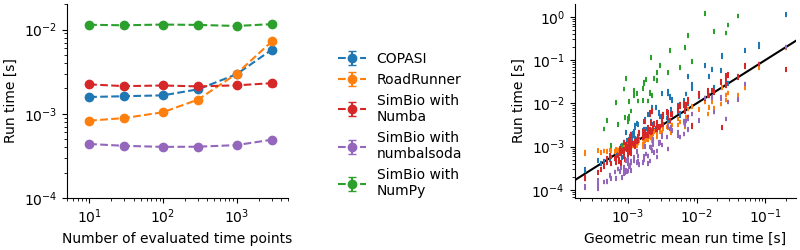
\includegraphics{src/performance/figures/performance.png}

}

\caption{\label{fig-runtime}Performance of different softwares to solve
models from the curated section of BioModels. (left) Run time for the
model BIOMD3 as a function of the number of output points. (right) Run
time for different models for 300 output points, using the geometric
mean of the different softwares to order them.}

\end{figure}


To evaluate SimBio's reproducibility, we analyzed curated SBML models
from BioModels (Malik-Sheriff et al. 2020). Among the first 100 curated
models from BioModels we selected 60 which did not contains events, as
SimBio doesn't support events yet. We simulated the selected models with
COPASI and used the simulated results as ground truth, and demonstrated
that SimBio reproduces the results with minor numerical differences
depending on the solver tolerance.

For performance testing, we ran simulations using COPASI,
Tellurium/RoadRunner, and SimBio. Within SimBio, both NumPy and Numba
backends were considered. The LSODA solver was used for COPASI and
SimBio, while for Tellurium the comparable CVODE solver was used. In all
cases, we used relative and absolute tolerances of \(10^{-6}\). We
measured three simulation stages: loading, the initial (cold) run, and
subsequent (warm) runs for each model.

For COPASI and Tellurium/RoadRunner, we noted that its runtime depended
on the number of evaluation points, something that does not seem to
happen with SimBio (Figure~\ref{fig-runtime}, left). While SimBio's
NumPy backend is slower than both COPASI and RoadRunner, we obtained an
order of magnitude speed-up using the numba backend putting it on par
with them. A user might have to consider the trade-off between
compilation and run times, as the compilation of the right-hand-side
(RHS) code might take longer than the runtime itself, and not be worth
it for running the model only once. Another speed-up in the runtime can
be had by switching the LSODA \texttt{scipy} solver for a more efficient
\texttt{numbalsoda} implementation, which avoids the Python interpreter
between each of the integration steps. This last combination beats all
other methods, which is also true for the other models we tested
(Figure~\ref{fig-runtime}, right).

\hypertarget{discussion}{%
\section{Discussion}\label{discussion}}

In this article, we introduced a suite of Python packages we developed
for defining and simulating dynamical systems and reaction networks.
These packages are deeply integrated with Integrated Development
Environments (IDEs), enabling code analysis tools to identify errors
prior to execution and assist in refactoring and code completion. We
adopted standard modern Python syntax to ensure seamless IDE
integration, supported by the extensive Python community.

Our approach differs from previous tools in that both the model
definition and its compilation into an Ordinary Differential Equation
(ODE) function are entirely Python-based. This approach simplifies the
development of various simulation methods, including performance
enhancements that exploit specific model structures. Importantly, being
Python-based does not compromise performance compared to C/C++ tools, as
the ODE functions can be Just-In-Time (JIT) compiled using Numba.

The inclusion of SBML support facilitates the effortless reuse of models
created by the systems biology community, along with the vast collection
of public models hosted in the BioModels repository. The modular
architecture of these packages facilitates their reuse, enhancement, and
extension by the wider Python community. For instance, an individual
from outside the systems biology field could contribute a stochastic
integrator to poincaré, which would then be available in SimBio. This
clear separation of concerns also makes the packages more
comprehensible, lowering the barrier for contributing improvements or
new features. Such an architecture ensures their maintainability and
ongoing development well into the future.

\hypertarget{resources}{%
\section{Resources}\label{resources}}

Source code repositories for these packages can be found at
\url{https://github.com/maurosilber/poincare} and
\url{https://github.com/hgrecco/simbio}.

\hypertarget{references}{%
\section{References}\label{references}}

\hypertarget{refs}{}
\begin{CSLReferences}{1}{0}
\leavevmode\vadjust pre{\hypertarget{ref-jax2018github}{}}%
Bradbury, James, Roy Frostig, Peter Hawkins, Matthew James Johnson,
Chris Leary, Dougal Maclaurin, George Necula, et al. 2018. {``{JAX}:
Composable Transformations of {Python}+{NumPy} Programs.''}

\leavevmode\vadjust pre{\hypertarget{ref-choiTelluriumExtensiblePythonbased2018}{}}%
Choi, Kiri, J Kyle Medley, Matthias König, Kaylene Stocking, Lucian
Smith, Stanley Gu, and Herbert M Sauro. 2018. {``Tellurium: {An}
Extensible Python-Based Modeling Environment for Systems and Synthetic
Biology.''} \emph{Bio Systems} 171 (September): 74--79.
\url{https://doi.org/10.1016/j.biosystems.2018.07.006}.

\leavevmode\vadjust pre{\hypertarget{ref-debontePEP681Data2021}{}}%
De Bonte, Erik, and Eric Traut. 2021. {``{PEP} 681 {\textendash} {Data
Class Transforms}.''} \emph{Python Enhancement Proposals}.
https://peps.python.org/pep-0681/.

\leavevmode\vadjust pre{\hypertarget{ref-harrisArrayProgrammingNumPy2020}{}}%
Harris, Charles R., K. Jarrod Millman, Stéfan J. van der Walt, Ralf
Gommers, Pauli Virtanen, David Cournapeau, Eric Wieser, et al. 2020.
{``Array Programming with {NumPy}.''} \emph{Nature} 585 (7825): 357--62.
\url{https://doi.org/10.1038/s41586-020-2649-2}.

\leavevmode\vadjust pre{\hypertarget{ref-harrisBioNetGenAdvancesRulebased2016}{}}%
Harris, Leonard A, Justin S Hogg, José-Juan Tapia, John A P Sekar,
Sanjana Gupta, Ilya Korsunsky, Arshi Arora, Dipak Barua, Robert P
Sheehan, and James R Faeder. 2016. {``{BioNetGen} 2.2: Advances in
Rule-Based Modeling.''} \emph{Bioinformatics (Oxford, England)} 32 (21):
3366--68. \url{https://doi.org/10.1093/bioinformatics/btw469}.

\leavevmode\vadjust pre{\hypertarget{ref-hoopsCOPASICOmplexPAthway2006}{}}%
Hoops, Stefan, Sven Sahle, Ralph Gauges, Christine Lee, Jürgen Pahle,
Natalia Simus, Mudita Singhal, Liang Xu, Pedro Mendes, and Ursula
Kummer. 2006. {``{COPASI}{\textemdash}a {COmplex PAthway SImulator}.''}
\emph{Bioinformatics} 22 (24): 3067--74.
\url{https://doi.org/10.1093/bioinformatics/btl485}.

\leavevmode\vadjust pre{\hypertarget{ref-huckaSBMLL3V2}{}}%
Hucka, Michael, Frank Bergmann, Stefan Hoops, Sarah M Keating, Nicolas
Le Novère, Chris J Myers, Brett G Olivier, et al. n.d. {``{SBML
L3V2}.''}

\leavevmode\vadjust pre{\hypertarget{ref-lamNumbaLLVMbasedPython2015}{}}%
Lam, Siu Kwan, Antoine Pitrou, and Stanley Seibert. 2015. {``Numba: A
{LLVM-based Python JIT} Compiler.''} In \emph{Proceedings of the {Second
Workshop} on the {LLVM Compiler Infrastructure} in {HPC}}, 1--6. {LLVM}
'15. {New York, NY, USA}: {Association for Computing Machinery}.
\url{https://doi.org/10.1145/2833157.2833162}.

\leavevmode\vadjust pre{\hypertarget{ref-lopezProgrammingBiologicalModels2013}{}}%
Lopez, Carlos F, Jeremy L Muhlich, John A Bachman, and Peter K Sorger.
2013. {``Programming Biological Models in {Python} Using {PySB}.''}
\emph{Molecular Systems Biology} 9 (January): 646.
\url{https://doi.org/10.1038/msb.2013.1}.

\leavevmode\vadjust pre{\hypertarget{ref-malik-sheriffBioModels15Years2020}{}}%
Malik-Sheriff, Rahuman S, Mihai Glont, Tung V N Nguyen, Krishna Tiwari,
Matthew G Roberts, Ashley Xavier, Manh T Vu, et al. 2020.
{``{BioModels}{\textemdash}15 Years of Sharing Computational Models in
Life Science.''} \emph{Nucleic Acids Research} 48 (D1): D407--15.
\url{https://doi.org/10.1093/nar/gkz1055}.

\leavevmode\vadjust pre{\hypertarget{ref-mckinneyDataStructuresStatistical2010}{}}%
McKinney, Wes. 2010. {``Data {Structures} for {Statistical Computing} in
{Python}.''} In \emph{Python in {Science Conference}}, 56--61. {Austin,
Texas}. \url{https://doi.org/10.25080/Majora-92bf1922-00a}.

\leavevmode\vadjust pre{\hypertarget{ref-meurerSymPySymbolicComputing2017}{}}%
Meurer, Aaron, Christopher P. Smith, Mateusz Paprocki, Ondřej Čertík,
Sergey B. Kirpichev, Matthew Rocklin, AmiT Kumar, et al. 2017.
{``{SymPy}: Symbolic Computing in {Python}.''} \emph{PeerJ Computer
Science} 3 (January): e103. \url{https://doi.org/10.7717/peerj-cs.103}.

\leavevmode\vadjust pre{\hypertarget{ref-shaikhBioSimulatorsCentralRegistry2022}{}}%
Shaikh, Bilal, Lucian P Smith, Dan Vasilescu, Gnaneswara Marupilla,
Michael Wilson, Eran Agmon, Henry Agnew, et al. 2022.
{``{BioSimulators}: A Central Registry of Simulation Engines and
Services for Recommending Specific Tools.''} \emph{Nucleic Acids
Research} 50 (W1): W108--14. \url{https://doi.org/10.1093/nar/gkac331}.

\leavevmode\vadjust pre{\hypertarget{ref-smithAntimonyModularModel2009}{}}%
Smith, Lucian P., Frank T. Bergmann, Deepak Chandran, and Herbert M.
Sauro. 2009. {``Antimony: A Modular Model Definition Language.''}
\emph{Bioinformatics} 25 (18): 2452--54.
\url{https://doi.org/10.1093/bioinformatics/btp401}.

\end{CSLReferences}



\end{document}
